% {{{
\documentclass[12pt]{article}
\usepackage[tmargin=0.75in,bmargin=0.75in,lmargin=0.9in,rmargin=0.9in]{geometry}

\usepackage{amsmath}
\include{latexsym}
\include{amssymb}
\usepackage{enumitem}
\usepackage[symbol, hang]{footmisc}
\usepackage{indentfirst}
\usepackage{amssymb}
\usepackage{graphicx,psfrag}

\def\F{\mathcal{F}}
\def\M{\mathcal{M}}
\def\dimspec{\mathfrak{D}}
\def\htop{h_{top}}
\def\trans{\mathcal{T}}
\def\G{\mathcal{G}}
\newcommand{\Z}{\mathbb{Z}}
\pagenumbering{gobble}
\def\O{\mathcal{O}}

\newcommand\NoIndent[1]{%
  \begingroup
  \par
  \parshape0
  #1\par
  \endgroup
}
% }}}

% Title {{{
\begin{document}

\begin{center}
{\large \bf Econ417 }   \\ \large Pset 3 \\ Ephraim Sutherland
\end{center}
% }}}

\subsection*{Problem 1}
% problem 1 {{{
\begin{enumerate}

\item we know that $c_0 = 0_0 - a_1$ 

	$$\max_{c_1, c_0} \; \log(c_0) + \beta \log(c_1)$$
	
	As in class we can rewrite this as a function of $a_1$

	$$\max_{a_1} \; \log(a_0 - a_1) + \beta \log(a_1)$$
	
	F.O.C. wrt $a_1$
	\begin{align*}
		\frac{-1}{a_0 - a_1} + \frac{\beta}{a_1} &= 0 \\
		a_1 = \frac{\beta a_0}{1 + \beta} &= c_1^* \\
		c_0^* = a_0 - a_1 &= a_0 - \frac{\beta a_0}{1 + \beta}
	\end{align*}
	The value function is 
	\begin{align*}
		v_2(a_0) &= \log(a_0 - \frac{\beta a_0}{1 + \beta}) + \beta \log(\frac{\beta a_0}{1 + \beta} ) \\
		       &= \log(a_0(1 - \frac{\beta}{1 + \beta})) + \beta \log(a_0) + \beta \log(\frac{\beta }{1 + \beta} ) \\
		       &= \log(1 - \frac{\beta}{1 + \beta}) + \log(a_0) + \beta \log(a_0) + \beta \log(\frac{\beta }{1 + \beta} ) \\
		       &= \log(1 - \frac{\beta}{1 + \beta}) + \beta \log(\frac{\beta }{1 + \beta} ) + (1 + \beta) \log(a_0)  \\
	\end{align*}

\item For the three period, recall we want

	\begin{align*}
		&\max_{a_1, a_2} \: \log(a_0 - a_1) + \beta \log(a_1 - a_2)  + \beta^2 \log(a_2)  \\
\iff 
&\max_{a_1, a_2} \: \log(a_0 - a_1) + \beta \left[ \log(a_1 - a_2)  + \beta \log(a_2)  \right ] \\
\iff 
&\max_{a_1} \: \log(a_0 - a_1) + \beta \left[ v_2(a_1) \right] \\
\end{align*}
F.O.C:

\begin{align*}
	\frac{-1}{a_0 - a_1} + \frac{\beta (1 + \beta)}{a_1} = 0 \\\\
	a_1 = \frac{\beta(1+\beta)}{(1 + \beta(1+\beta))} a_0 = \frac{\beta+\beta^2}{(1 + \beta+\beta^2)} a_0
\end{align*}
next 
$$\max_{a_2} \log(a_1 - a_2) + \beta \log(a_2)$$
FOC:
\begin{align*}
	\frac{-1}{a_1 - a_2} + \frac{\beta}{a_2} = 0 \\
	\frac{1}{a_1 - a_2} = \frac{\beta}{a_2}  \\
	a_2 = \frac{\beta}{(1+ \beta)}a_1 \\
	    = \frac{\beta}{(1+ \beta)} \frac{\beta(1+\beta)}{(1 + \beta(1+\beta))} a_0 \\
	    = \frac{\beta^2}{(1 + \beta +\beta^2)} a_0 
\end{align*}
Thus 
\begin{align*}
&c_0^* = a_0^* - a_1^* = \frac{1}{(1 + \beta +\beta^2)} a_0 \\
&c_1^* = a_1^* - a_2^* = \frac{\beta+\beta^2}{(1 + \beta+\beta^2)} a_0 - \frac{\beta^2}{(1 + \beta +\beta^2)} a_0 = \frac{\beta}{(1 + \beta +\beta^2)} a_0 \\
&c_2^* = a_2^* = \frac{\beta^2}{(1 + \beta +\beta^2)} a_0
\end{align*}

We can then get the value function 
\begin{align*}
	v_3^* ( a_0) &= \log(\frac{a_0}{(1 + \beta +\beta^2)} ) + \beta \log(\frac{a_0 \beta}{(1 + \beta +\beta^2)} ) + \beta^2 \log(\frac{a_0 \beta^2}{(1 + \beta +\beta^2)} ) \\
		     &= \log(a_0) - \log(1 + \beta + \beta^2) + \beta \log(\beta) + \beta\log(a_0) - \beta \log(1 + \beta + \beta^2) + \\
		     & \beta^2 \log(a_0) + \beta^2 \log(\beta^2) - \beta^2\log(1 + \beta + \beta^2)
\end{align*}
let $A$ be a constant which represents the terms which are not a function of $a_0$ then we have that
$$v_3^* ( a_0) = A + (1 + \beta + \beta^2) \log(a_0)$$

\item we know we want to solve
	\begin{align*}
		\max_{a' \in [0,a]} \left[\log(a - a') + \beta ( \gamma_0 + \gamma_1 \log(a')) \right]
	\end{align*}
	solving FOC, we get:
	\begin{align*}
		\frac{-1}{a - a'} + \frac{\beta \gamma_1}{a'} = 0 
	\end{align*}
	Solving for $a'$ we get
	$$a' = \frac{\beta \gamma_1}{(1 + \beta \gamma_1)} a $$
	Now to get the value function,
	we have that 
	\begin{align*}
		v(a) &= \log(a - \frac{\beta \gamma_1 a}{(1 + \beta \gamma_1)} ) + \beta v(\frac{\beta \gamma_1 a}{(1 + \beta \gamma_1)} ) \\
		     &= \log(\frac{a}{(1 + \beta \gamma_1)} ) + \beta \left(\gamma_0 + \gamma_1 \log(\frac{\beta \gamma_1 a}{(1 + \beta \gamma_1)}  \right) \\
		     &= - \log(1 + \beta \gamma_1) + \beta \left( \gamma_0 + \gamma_1 \log(\frac{\beta \gamma_1 }{(1 + \beta \gamma_1)}  \right)  + (1 + \beta \gamma_1) \log(a)
	\end{align*}
	Now clearly we can choose $\gamma_1' = (1 + \beta \gamma_1)$ and $\gamma_0' = - \log(1 + \beta \gamma_1) + \beta \left( \gamma_0 + \gamma_1 \log(\frac{\beta \gamma_1 }{(1 + \beta \gamma_1)}  \right)$  and we have the desired form.
      Now simply set  $\gamma_1 = \gamma_1'$ and we get
      \begin{align*}
      	\gamma_1 = \gamma_1' = 1 + \beta \gamma_1 \iff \gamma_1 = \frac{1}{1 - \beta}
      \end{align*}
      This is also what we'd expect from the geometric sum that seems to be arising.

      For $\gamma_0$, again
      \begin{align*}
	      \gamma_0 &= \gamma_0' \\
		       &= - \log(1 + \beta \gamma_1) + \beta \left( \gamma_0 + \gamma_1 \log(\frac{\beta \gamma_1 }{(1 + \beta \gamma_1)}  \right) \\
		       &= - \log( \gamma_1) + \beta \gamma_0 + \gamma_1 \beta \log(\beta ) \\
	      \iff (1 - \beta) \gamma_0 &= \log(1 - \beta) + \frac{\beta}{1 - \beta} \log(\beta) \\
		      \iff \gamma_0 &= \frac{1}{1 - \beta} \log(1 - \beta) + \frac{\beta}{(1 - \beta)^2} \log(\beta)
      \end{align*}

      \item for optimal decision rule we then get
	      \begin{align*}
		      a' &= g(a) = \frac{\beta \gamma_1}{(1 + \beta \gamma_1)} a \\
	      &= \frac{\frac{\beta}{1 - \beta}}{\frac{1}{1 - \beta }} a \\
	      & = \beta a
      \end{align*}
In other words, in every period, the consumer saves $\beta$ of the good to bring into the next period.
Thus $a_t = \beta^t a_0$. We can then also clearly see that the consumer will eventually run out of cake because we know  $0 <\beta < 1$ so it follows that  $\lim_{t \to \infty} a_t = 0$
\end{enumerate} 

% }}}

% Problem 2 {{{
\subsection*{Problem 2}

\begin{enumerate}
	\item coded in Q2.jl

		\begin{center}
			\textbf{a}\par\medskip
			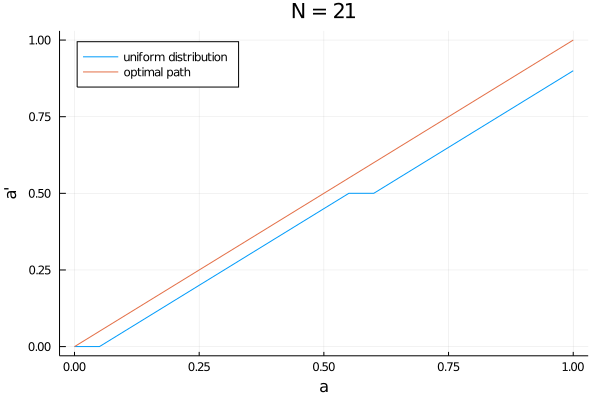
\includegraphics[width=0.8\linewidth]{plot_a1.png}
			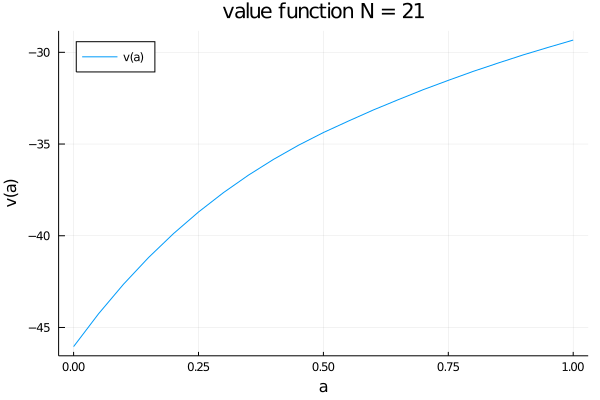
\includegraphics[width=0.8\linewidth]{plot_v1.png}
		\end{center}
	\item 

		\begin{center}
			\textbf{b}\par\medskip
			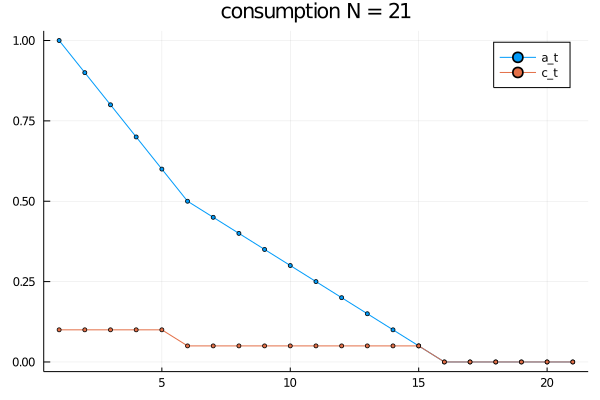
\includegraphics[width=0.8\linewidth]{plot_c1.png}
		\end{center}

	\item
		\begin{center}
			\textbf{a}\par\medskip
			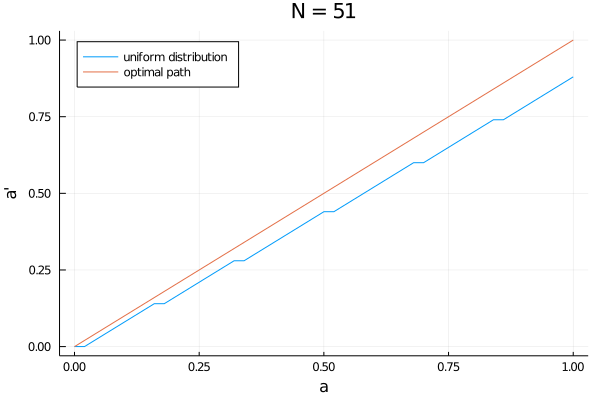
\includegraphics[width=0.8\linewidth]{plot_a2.png}
			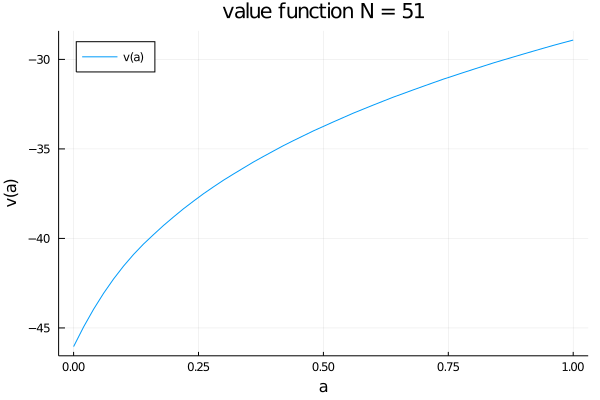
\includegraphics[width=0.8\linewidth]{plot_v2.png}
		\end{center}
	\item 

		\begin{center}
			\textbf{b}\par\medskip
			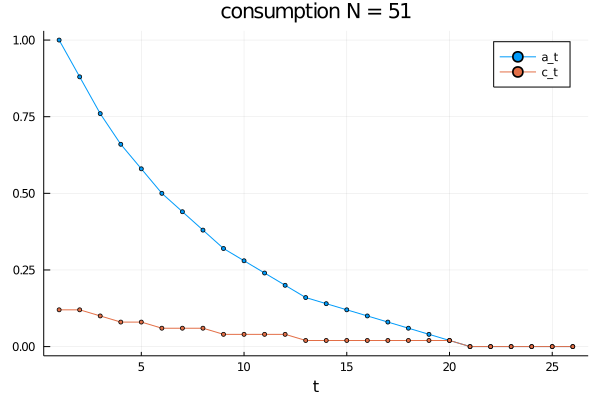
\includegraphics[width=0.8\linewidth]{plot_c2.png}
		\end{center}
\end{enumerate}

% }}}
\end{document}


